%*****************************************************************
%*************************** Section 8 ***************************
%************************ Verteilerplatine ***********************
%*****************************************************************


\pagestyle{fancy}
\rhead{\thepage} \chead{} \lhead{\ref{Sec8}. \nameref{Sec8}}
\cfoot{}

\section{Verteilerplatinen}\label{Sec8}

Anders als beim Fahrzeug von Herrn Arne Kullina werden bei dieser Fahrzeugversion zwei statt nur einer Verteilerplatine verbaut. Die Leistungsverteilung findet auf der Grundplatte platz und die steckbare Verteilung der Signale für die Fahrzeugperipherie auf der oberen Ebene. 

\subsection{Leistungsverteiler auf der unteren Fahrzeugebene}\label{Sec8Sub1}

\begin{minipage}[t]{0.47\textwidth}
Von der Stromverteilerplatine auf der unteren Fahrzeugebene aus (siehe Abbildung \ref{fig:Stromverteilerplatine}) wird die gesamte Fahrzeugperipherie mit der Batteriespannung versorgt. Sowohl der Schaltspannungsregler, als auch der Linearspannungsregler auf der oberen Verteilerplatine und die \acp{ESC} erhalten hier ihre Versorgungsspannung. Der Vorteil, dass auf der Grundplatte lediglich der Versorgungsspannungsabgriff erfolgt liegt darin, dass das Fahrzeug seltener zerlegt werden muss. Da auf der Grundplatte keine wichtige Hardware-Schaltung platz findet, können die meisten Probleme gelöst werden, ohne auf die untere Fahrzeugebene zugreifen zu müssen.
\end{minipage}
\begin{minipage}[t]{0.47\textwidth}
\vspace{-7mm}
\begin{figure}[H] %H für Positionierung hier
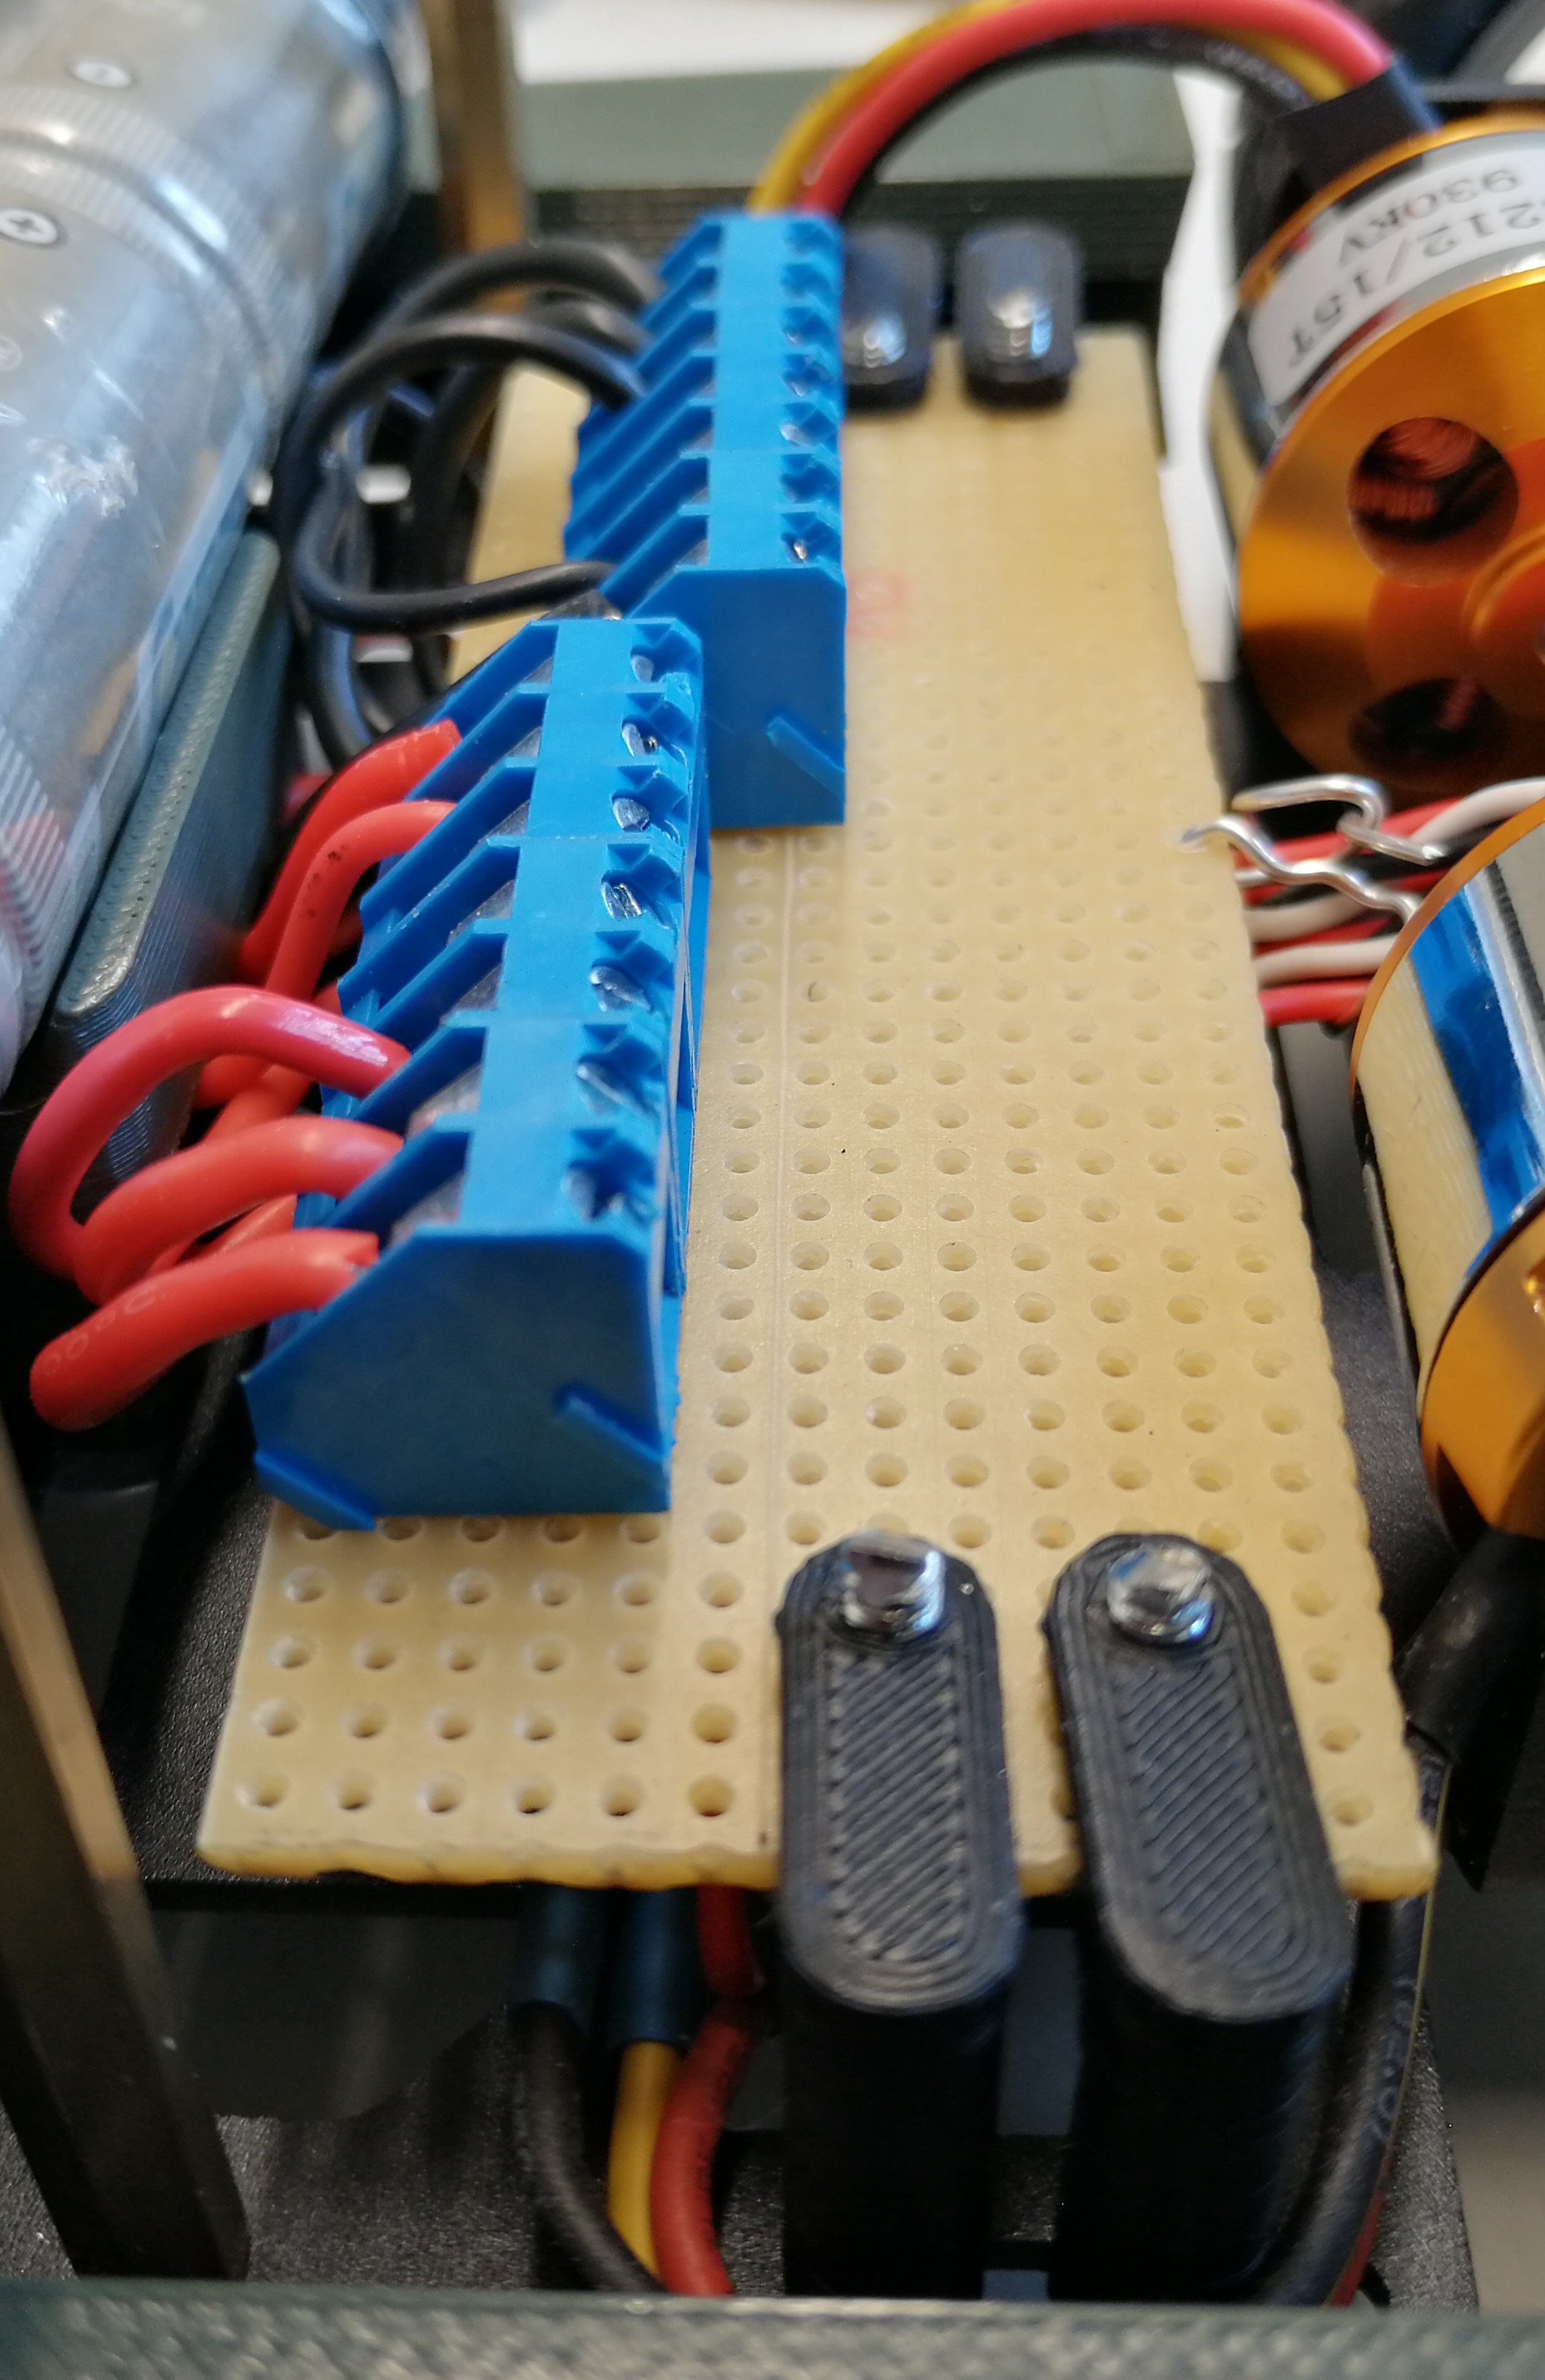
\includegraphics[width=.7\textwidth]{sec8/images/Leistungsverteilerplatine} 
\centering
\captionsetup{width=.9\textwidth}
\caption[Leistungsverteilerplatine auf der unteren Fahrzeugebene]{Leistungsverteilerplatine auf der unteren Fahrzeugebene}
\centering
\label{fig:Leistungsverteilerplatine}
\end{figure}
\end{minipage}


\subsection{Signalverteilerplatine auf der oberen Fahrzeugebene}\label{Sec8Sub2}


\begin{figure}[H] %H für Positionierung hier
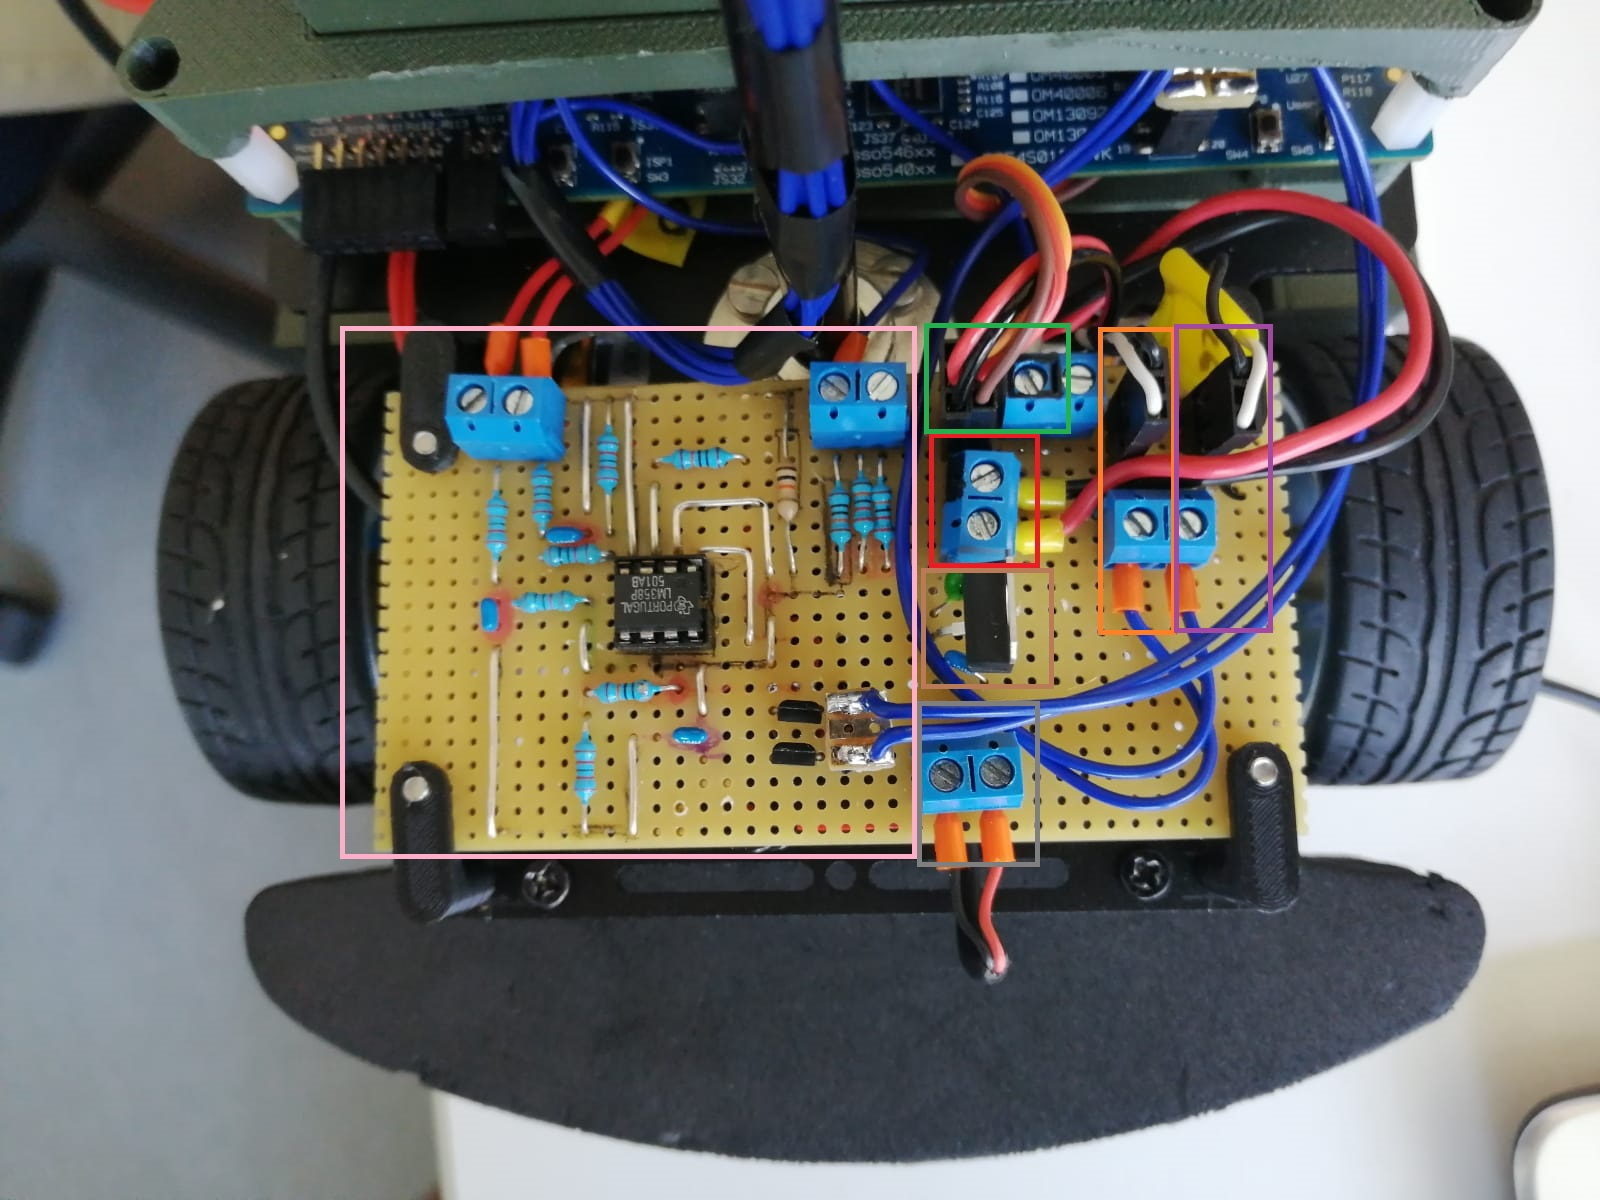
\includegraphics[width=.7\textwidth]{sec8/images/Signalverteilerplatine} 
\centering
\captionsetup{width=.9\textwidth}
\caption[Signalverteilerplatine auf der oberen Fahrzeugebene]{Signalverteilerplatine auf der oberen Fahrzeugebene}
\centering
\label{fig:Signalverteilerplatine}
\end{figure}


\newpage